%------------------------------------------------------------------------------

\documentclass{uofsthesis-cs}

\usepackage[pdftex]{graphicx}
\usepackage{pdfpages}

%------------------------------------------------------------------------------

% THESIS TITLE
\title{Play Experience Enhancement Using Emotional Feedback}

% AUTHOR'S NAME
\author{Faham Negini}

% DEGREE SOUGHT
\degree{\MSc}

% EXPECTED CONVOCATION DATE
\convocationdate{September/2013}

% NAME OF ACADEMIC UNIT
\department{Computer Science}
% \academicunit{Division}

% PERMISSION TO USE ADDRESS
\ptuaddress{Head of the Department of Computer Science\\
176 Thorvaldson Building\\
110 Science Place\\
University of Saskatchewan\\
Saskatoon, Saskatchewan\\
Canada\\
S7N 5C9
}

%------------------------------------------------------------------------------

\abstract          {% Abstract less than or equal to 1 page
% one page stating what the thesis is about
% highlight the contributions of the thesis

Innovations in computer game interfaces continue to enhance the experience of players. Affective games –those that adapt or incorporate a player’s emotional state – have shown promise in creating exciting and engaging user experiences. However, a dearth of systematic exploration into what types of game elements should adapt to affective state leaves game designers with little guidance on how to incorporate affect into their games. We created an affective game engine, using it to deploy a design probe into how adapting the player’s abilities, the enemy’s abilities, or variables in the environment affects player performance and experience. Our results suggest that affectively adapting games can increase player arousal. Furthermore, we suggest that reducing challenge by adapting non-player characters is a worse design choice than giving players the tools that they need (through enhancing player abilities or a supportive environment) to master greater challenges.}
\acknowledgements  {First and foremost thanks God for bestowing me the ability to learn, to speak and to write. For all of the oppurtinities and all of His mercy and compassion I have experienced throughout my life.\\

I would like to express my sincere gratitude to my advisors Prof. Regan Mandryk  and Prof. Kevin G. Stanley for the continuous support of my M.S. study and research, for their patience, motivation and friendliness. Their guidance helped me in all the time of research and writing of this thesis. I could not imagine having any better advisors and mentors for my M.S. study.\\

Besides my advisors, I would like to thank the rest of my thesis committee: Prof. , Prof. , and Dr. , for their encouragement, insightful comments, and hard questions.\\

My sincere thanks also goes to Dr. Daniel Neilson, Gwen Lancaster, Shakiba Jalal and Dr. Stanley for offering me the internship opportunities and leading me working on diverse exciting projects.\\

I would like to thank my wife Farzane Jenaban for her pacience, understanding and support in every single moment my attention was away from her towards this research and thesis; And my parents Mohammad Negini and Farzaneh Sarmadi, for their spiritual support throughout my life.\\

Last but not the least I thank my fellow labmates in DISCUS and HCI Labs: Mohammad Hashemian, Amin Tavassolian, Ariyan Zohoorian, Farjana Eishita, Max Birk, Michael Kalyn, Michael Bullock and Steve Sutcliffe, for the stimulating discussions, for the nights we were working together, and for all the fun we have had in the last years. Also I thank all of my other friends in University of Saskatchewan.\\
}
%\dedication       {This is the thesis dedication (optional)}
\loa               {\abbrev{TT}   {Thought Technology}
\abbrev{GSR}  {Galvanic Skin Response}
\abbrev{EMG}  {Electromyography}
\abbrev{EKG}  {Electrocardiography}
\abbrev{ECG}  {Electrocardiography}
\abbrev{HF}   {High-frequency}
\abbrev{HR}   {Heart Rate}
\abbrev{HRV}  {Heart Rate Variability}
\abbrev{BVP}  {Blood Volume Pulse}
\abbrev{EDA}  {Electrodermal Activity}
\abbrev{HCI}  {Human Computer Interaction}
\abbrev{AV}   {Arousal/Valence}
\abbrev{NPC}  {Non-Player Character}
\abbrev{Mod}  {Modification}
\abbrev{CSV}  {Camma Separated Values}
\abbrev{SAM}  {Self-Assessment-Manikin}
\abbrev{PENS} {Player Experience of Need Satisfaction}
\abbrev{IMI}  {Intrinsic Motivation Inventory}
\abbrev{GEQ}  {Game Engagement/Experience Questionnaire}
\abbrev{ICU}  {Intensive Care Unit}
\abbrev{FPS}  {First-Person Shooter}
\abbrev{EDR}  {Electrodermal Response}
\abbrev{EDA}  {Electrodermal Activity}
}

%------------------------------------------------------------------------------

\begin{document}

% Typeset the title page
\maketitle

% Typeset the frontmatter.
\frontmatter

%------------------------------------------------------------------------------


%------------------------------------------------------------------------------

%\img
%{caption}
%{description}
%{file path reltive to images/}
%{label}

\newcommand{\img}[4]{
\begin{figure}[h]
  \caption[#1]{#2}
  \centering
  \includegraphics[width=0.5\textwidth]{images/#3}
  \label{fig:#4}
\end{figure}
}

%------------------------------------------------------------------------------

\newcommand{\bhline}{\specialrule{.1em}{.05em}{.05em}}

%------------------------------------------------------------------------------
 %new commands go here


%------------------------------------------------------------------------------

\chapter{Introduction}
\label{chap:intro}

% 5 to 10 pages
% Thesis Statement (one or two sentences)
% What is your thesis about and what have you done?
% If you have a hypothesis what is it?
% How will you test (prove/disprove) your hypothesis?
% Motivation
% Why is this problem you've worked on important
% Goals / Objectives
% What are you trying to do and why?
% How will you or the reader know if or when you've met your objectives?
% **** Contributions *****
% What is new, different, better, significant?
% Why is the world a better place because of what you've done?
% What have you contributed to the field of research?
% What is now known/possible/better because of your thesis?
% Outline of the thesis (optional)

Since computers are playing a significant role in our daily life, the need for a more friendly and natural communication interface between human and computer has continiously increased. Making computers capabale of perceiving the situation in terms of most human specific factors and responding dependent to this perception is of major steps to acquire this goal. If computers could recognize the situation the same way as human does, they would be much more natural to communicate. Emotions are of important and mysterious human attributes that have a great effect on people's day to day behavior. Researchs from neuroscience, psychology, and cognitive science, suggests that emotion plays critical roles in rational and intelligent behavior ~\cite{picard2001toward}. Apparently, emotion interacts with thinking in ways that are nonobvious but important for intelligent functioning ~\cite{picard2001toward}. Scientists have amassed evidence that emotional skills are a basic component of intelligence, especially for learning preferences and adapting to what is important ~\cite{mayer1993intelligence, goleman2006emotional} People used to express their emotions through facial expressions, body movement, gestures and tone of voice and expect others understand and answer to their affective state. But sometimes there is a distinction between inner emotional experiences and the outward emotional expressions ~\cite{picard2003affective}. Some emotions can be hard to recognise by humans, and inner emotional experiences may not be expressed outwardly ~\cite{jones2007biometric}. Recent extensive investigations of physiological signals for emotion detection have been providing encouraging results where affective states are directly related to change in inner bodily signals ~\cite{jones2007biometric}. However whether we can use physiological patterns to recognise distinct emotions is still a question ~\cite{picard2001toward, cacioppo1990inferring}.

Although the study of affective computing has increased considerably during the last years, few have applied their research to play technologies ~\cite{sykes2003affective}. Emotional component of human computer interaction in video games is surprisingly important. Game players frequently turn to the console in their search for an emotional experience ~\cite{rouse2010game}. There are numerous benefits such technology could bring video game experience, like: The ability to generate game content dynamically with respect to the affective state of the player, the ability to communicate the affective state of the game player to third parties and adoption of new game mechanics based on the affective state of the player ~\cite{sykes2003affective}. This work concentrates on developing a real-time emotion recognition system for play technologies which can quantify player instant emotional state during a play experience The rest of the paper is organized as follows: in Section 2 we outline different emotion recognition theories with an overview of physiology sensors. In Section 3 we demonstrate some implementation details of the system. We then describe the experimental setup in Section 4 before giving our results in Section 5. Finally, we give conclusions in Section 6.

%------------------------------------------------------------------------------

\chapter{Human and Play Technologies}
\label{chap:man-n-play}

%8 to 20 pages around 50 to 70 ref
%More than a literature review
%Organize related work - impose structure
%Be clear as to how previous work being described relates to your own.
%The reader should not be left wondering why you've described something!!
%Critique the existing work - Where is it strong where is it weak? What are the unreasonable/undesirable assumptions?
%Identify opportunities for more research (i.e., your thesis) Are there unaddressed, or more important related topics?
%After reading this chapter, one should understand the motivation for and importance of your thesis
%You should clearly and precisely define all of the key concepts dealt with in the rest of the thesis, and teach the
%reader what s/he needs to know to understand the rest of the thesis.

%%% 1 page: overview of what is going on

In this chapter, related research to this work is being presented. It starts with introducing and reviewing common terminology used in the research on affect and emotion and the methods that have been used to measure affect and emotion; And continues by presenting previous research in game balancing that inspired this work in its game experience enhancement study.

\section{Affect and Emotion}

In this section common terms used in the literature is introduced along with different ways these terms are often described.

\subsection{Terminology}

The terms \textit{affect} and \textit{emotion} are often used interchangeably and using these terms without any specific description highlighting their differences can be usually confusing. To avoid this confusion it is important to understand the distinction between these terms. In this thesis, \textit{affect} is used in a more general sense that encompasses emotions ~\cite{forgas1995mood} while \textit{emotions} are usually reactionary fealings often triggered by some particular cause either physical or cognitive and are short in duration; Individuals are usually aware of the presence of an emotion ~\cite{paiva2007affective}.

Classical attempts to describe emotion can be categorized into two major different approaches: Those that try to describe emotion by emphasizing its cognitive (mental) aspects and those that concentrate on its bodily (physical) aspects. Walter Cannon by suggesting emotion as an experience within the brain, independent of the sensations of the body ~\cite{cannon1927james} is usually credited for the cognitive approach. On the other hand the physical approach has largely been attributed to William James in which physiological responses (e.g. elevated heart rate) are the center of focus that occurs just prior or during an emotional episode ~\cite{paiva2007affective}.

In more recent approaches emotion has been considered as a combined result of cognitive and physiological changes simultaneously. ~\cite{paiva2007affective}. Body chemistry changes and thoughts can both contribute to the definition of emotions; As Schachter suggests emotion is our interpretation of a specific physiological reactions along with our mental situation that is labeled as an emotion (e.g. fear) ~\cite{schachter1964interaction}. In this thesis, \textit{emotional state} refers to the combinational internal dynamics (both cognitive and physiological) that are perceived by an individual during an emotional experience ~\cite{paiva2007affective}.

\section{Describing Emotion}

Identifying emotions by dividing them into discrete categories or assuming a continuous dimensional space in which emotions can be defined are two major approaches that the related research has gone into to describe emotions.

\subsection{Discrete Categories}

Suggested discrete categories in the categorical approach does not necessarily agree with one another. This approach, also known as the basic emotion theory largely relies on language in its mission to describe emotion; In fact, it begins by identifying specific labels people attach to different emotional episodes and then suggests categories of emotions. Examples of such labels (or categories) include excitement, anger, fear, sadness and happiness. Relying on language to describing emotions not only led suggested categories to vary across languages, but also within a language. The variability and disagreement in the literature suggests a lack for clear definitions or boundaries for these states, which has caused difficulties when comparing different research approaches. In-availability of specific categories in other languages also makes research using this approach difficult ~\cite{zimmermann2006extending}

Recent works on the basic emotion theory identifies anger, disgust, fear, happiness, sadness, and surprise ~\cite{peter2006emotion} as the concise set of primary emotions. These are actually the least six universal categories researchers agreed upon ~\cite{zagalo2004story}. It also claims these primary emotions are distinguishable from each other and other affective phenomena ~\cite{dalgleish1999handbook}.

\subsection{Continuous Dimensions}

The dimensional emotion theory argues that all emotional states reside in a two-dimensional space, defined by arousal and valence. This approach described by Russell in ~\cite{russell2003core} introduces the idea of core affect to identify emotions. It holds core affect accountable for feelings triggered by specific events and describes it as being composed of two independent dimensions: arousal and valence. Figure ~\ref{fig:russel-av-space} illustrates the concept of arousal and valence space describing various emotions known as common emotion categories.

\img
{Russell's arousal and valence model}
{Russell's circumplex model with two axes of arousal and valence \footnotemark.}
{russell-av-space.pdf}
{russel-av-space}
\footnotetext{Photo credit: http://imagine-it.org/gamessurvey/}

The energy or the degree of activation of an individual which brings a sense of mobilization is usually referred to as \textit{arousal}. The arousal state is physiological and psychological state of being reactive and responsive to a stimuli. The flight-or-fight response, as introduced in Cannon's theory ~\cite{stern2001psychophysiological} is a physiological reaction that occurs in response to a perceived threat or stimuli and focuses on the physiological changes that occur in the body during these situations. Different qualities of arousal are usually studied as low (e.g. sleepiness) to high (e.g. excitement).

Valence as often used in psychology particularly in study of emotions, means the intrinsic attractiveness (positive valence) or aversiveness (negative valence) of an event or situation ~\cite{frijda1986emotions}. However in many related studies of emotion, the term is also used to identify popular emotions by their negative or positive impressions. Emotions with lower valence are those that are less desired such as anger and fear, and emotions with higher valence are those that are more desired such as joy and happiness.

\section{Recognizing Emotions}

In this work, both the categorical and dimensional approaches are used for developed models. The model developed for capturing emotional state responses is coupled with gathered subjective emotional experiences of our participants based on a categorical approach. Using categorical approach when collecting emotional experiences subjectively is the most practical method, as it is far easier for participants to communicate in a language that they can understand (emotional categories rather than the degree of arousal or valence) to describe their emotional state best. However although we did not want to use a data collection process that require the participants to learn new terminologies and describe their emotional estate with unfamiliar terms, participants have been introduced to arousal, valence and dominance. Given example emotions for different levels of these variables participants tried to describe their affect state by choosing images based on these concepts. The developed model for the affect space uses the dimensional model as in Figure ~\ref{fig:russel-av-space} to provide a mapping between the original emotional categories and a dimensional space. These models are further elaborated in Chapter ~\ref{chap:impl}.

 ~\cite{picard2003affective}

p There are many different emotional indicators that have been studied to determine affect including facial expressions, gestures, postures, vocal intonation, language, pressure, and pupil dilation [45]. These are all visible features that can be observed by others through day-to-day interactions. For example, in human-to-human interactions, facial expression can help us to determine whether someone is distracted, frustrated, or happy just through facial expression. Some researchers have used sophisticated face-tracking software to analyze facial expressions to infer the emotional state of the user [11,44]. Work by Khan et al. [31] extended this idea but used thermal imaging to identify changes of blood flow patterns in the face that correspond to different facial expressions. 

p There are also a number of other indicators that are less visible to another person, such as physiological changes in the body that occur during emotional episodes. In [38], Mandryk et al. used physiological metrics such as galvanic skin response (GSR), respiration, electrocardiography (EKG), and electromyography of the jaw (EMG) as indicators of participants‘ affective states while playing video games. These indicators are measured through electronic sensors placed directly on the skin, face, chest, and hands of the participant.



While there are various opinions on identifying emotional states, classification into discrete emotions ~\cite{dalgleish1999handbook}, or locating emotions along multiple axes ~\cite{russell1989affect, lang1995emotion}, both had limited success in using physiology to identify emotional states ~\cite{cacioppo2000psychophysiology}.

Lang used a 2-D space defined by arousal and valence (pleasure) (AV space) to classify emotions ~\cite{lang1995emotion}. Valence can be described as a subjective feeling of pleasantness or unpleasantness while arousal is the subjective state feeling activated or deactivated ~\cite{barrett1998discrete}. Using an arousal-valence space to create the Affect Grid, Russell believed that arousal and valence are cognitive dimensions of individual emotion states. Affect is a broad definition that includes feelings, moods, sentiments etc. and is commonly used to define the concept of emotion ~\cite{picard2003affective}. Russell's model has two axes that might be labeled as displeasure/pleasure (horizontal axis) and low/high arousal (vertical axis) It is not easy to map affective states into distinctive emotional states, However these models can provide a mapping between predefined states and the level of arousal and valence ~\cite{zagalo2004story}, Figure ~\ref{fig:russel-av-space}.


Both mentioned models for identifying emotions convey some practical issues in emotion measurement. In a HCI context, the stimuli for potential emotions may vary less than in human-human interaction (e.g., participant verbal expressions and body language) ~\cite{zhang2010service} and also the combination of evoked emotions ~\cite{peter2006emotion}. However with help of physiological signals and the fuzzy logic in the model we are going to use, such issues with our dimentional emotion models would be minimized. Though it is anticipated to observe different range of evoked emotions while interacting with play technologies compared to interacting with other humans in daily life. ~\cite{zhang2010service}. However our dimensional emotion models suffers some other problems. One problems is that arousal and valence are not independent and one can impact the other ~\cite{mandryk2007fuzzy}. Continuously capturing emotional experiences in this applied setting is of its other hallmarks. Subjective measures based on dimensional emotion theory, such as the Affect Grid ~\cite{russell1989affect} and the Self-Assessment Manikin ~\cite{bradley1994measuring}, allow for quick assessments of user emotional experiences but they may aggregate responses over the course of many events ~\cite{zhang2010service}. This work uses Mandryk et al. version of AV space ~\cite{mandryk2007fuzzy}.

Using emotional responses to increase the level of users interaction with a real-time play technology requires an effective technique to identifying specific emotion states within an emotional space. Major existing emotion models in the psychology literature includes: basic emotion theory ~\cite{ekman1992argument, ekman1992there} , dimensional emotion theory ~\cite{lang1995emotion, russell1980circumplex} and models from appraisal theory (e.g.,~\cite{roseman2001model}) ~\cite{zhang2010service}


\section{Measuring Affect}
%%% Talk about various sensors and their attributes, in particular the GSR sensor
%%% and how it can be used to detect Arousal using the fuzzy logic

p EKG measures the electrical activity of the heart which is measured on the surface of the skin using electrodes. These electrodes are commonly placed on the chest, forearm, or legs and are applied with conductive gels on the bare skin of the person being examined. The area where the electrodes are placed must be free of hair so shaving these regions may be necessary to prevent interference with the sensors [50].  

p Respiration measures the rate or volume of air exchange in the lungs. Although accurate results can be obtained by measuring gas exchange, the apparatus that is required (a face mask) prevents the user from speaking and requires them to remain stationary during the measurement process. Alternatively, measuring chest cavity expansion can also be used for these metrics using less obtrusive sensors (e.g. stretch sensor around the chest of the participant) [50].  

p The major problem with the physiological approaches to measuring affect is the intrusive nature of the technology. Affixing sensors to users‘ skin would not be realistic in a real-world context (e.g. casual interactions with mobile phones). Sensors take time to attach to the user, conductive gels might be used, shaving may be necessary, and the sensors can be sensitive to movement and could fall off with activity. Furthermore, the presence and constant reminder of the sensors may alter the emotional state that the user would have been in, if the sensors were not present. 

p Some physiological approaches to detecting emotional states are less obtrusive because they do not require physical contact with the participant. For example, thermal cameras have been leveraged to identify increased blood flow in particular regions of the face when the user is experiencing emotional states such as stress [46]. Although this type of technology is not as obtrusive as some of the other physiological approaches (such as GSR), the main drawback is that the approach requires the use of expensive technology (a thermal camera) that is not widely used in typical computer settings such as the home or office. This is also typical of the other physiological sensors previously mentioned (e.g. GSR) because they require specialized equipment that can be expensive, which limits the applicability of widespread adoption of this approach. 


\section{The Concept of Flow in Video Games}

\subsection{Challenge vs. Skill}

\img
{Russell's arousal and valence model}
{Mental state in terms of challenge level and skill level, according to Csikszentmihalyi's flow model ~\cite{csikszentmihalyi1997finding}}
{challenge-vs-skill.png}
{challenge-vs-skill}

\section{Emotionally Adaptive Games}
%%% talk about play technologies and why do people play them
%%% the importance of being challenged in play technologies
%%% and its effect on arousal level

%% olesen2008real
Computer game balance (or difficulty adjustment) is a
crucial aspect of commercial game development. Currently,
this is achieved either by predefined levels of game challenge
— the player then decides which of those levels she will play
against — or by techniques known as rubber-band artificial
intelligence (AI) [1], mainly used in racing games. The
first approach cannot incorporate the needs of all potential
players of the game while the latter approach generates
predictable behaviors which reduce the believability of the
non-player characters (NPCs). Furthermore, human players
enhance their skills while playing a game which necessitates
an adaptive mechanism that covers the player’s need for more
challenging NPCs during play (i.e. in real-time).
%% olesen2008real

%% TODO:paraphrase
For creating entertaining computer games1, gameplay is considered to be of key im- portance ([1], [2]). In absence of a broadly accepted definition of gameplay, we focus here on one frequently mentioned element of it, which is challenge. The process of optimizing a game’s challenge is referred to as game balancing or difficulty scaling. That is, changing parameters in order to avoid that the player gets frustrated because the game is too hard, or gets bored because the game is too easy [3]. In this study, we have investigated the relations between a game's difficulty level and the interplay between the emotions boredom, frustration and enjoyment (Fig. 1-left panel). These 
relations strongly differ per individual, for example influenced by a player's skill level. For instance, a difficulty level that is found enjoyable by a novice might be boring for expert players. Games therefore need psychological customization tech- niques [4], such as difficulty adaptation, to optimize the experience. Since many years, game designers aim to provide some customization, for example by letting players choose a difficulty level upfront or including progressive difficulty levels during gameplay, based on a player’s performance.   More advanced methods that work in real-time are less common. One difficulty adaptation mechanism, frequently applied in racing games, is called rubber banding [5]: When falling behind, the player suddenly gets an enormous boost in speed, which allows for catching up again (and vice versa for the competing cars). However, game adaptation that is solely based on in-game behavior can only have limited success, because there are many different types of players [6]. Each type of player has his/her own goals, preferences and emotional responses when playing a game. Hence, for optimizing the players' experiences, successful psychological customization requires a game to take the emotional state of the player into account. Games should become emotionally adaptive (Fig. 1– right panel). 

\img
{Emotionally adaptive games}
{Left panel: Game balancing (Adapted from [1]). Right panel: The emotionally adaptive games loop, inspired on the affective loop [7]. }
{adaptive-games.png}
{adaptive-games}

The importance of emotions in computing is widely argued for (e.g. [8]). Emotion theorists differ over a discrete versus a dimensional model. The \"discretionists\" (e.g. [9]) argue for basic discrete emotions, such as anger, fear, sadness and happiness, as unique experiential states. The \"dimensionalists\" (e.g. [10]), on the other hand, look at emotions in terms of a two-dimensional space consisting of valence ("pleasantness") and arousal ("activation"). Sometimes dominance is added as a third dimension.  Effective human-computer interaction from an emotions perspective works in terms of an \"affective loop\" [7]. A similar feedback loop in a games context is de- scribed by [11]. Inspired by their work, Fig. 1 (right panel) shows a schematic view on the functioning of an emotionally adaptive game. By providing the right game mechanics [12] (e.g. audiovisuals, narrative, challenge), the game influences the player's experience, behavior and emotional state. Ideally, during play, the emotional state of the player (measured in terms of emotion-data), is continuously being fed back to the game so that the game can adapt its mechanics (e.g. difficulty level)
accordingly in real-time. This all is done to create the optimal experience (which is referred to in literature as e.g. flow [13] or immersion [14]). Previous research at- tempts to create emotionally adaptive software have mainly focused on tutoring sys- tems and workload / performance optimization (see e.g. [15]). Fewer attempts have been made to incorporate a closed-loop mechanism in a games context. Takahashi et al. [16] and Rani et al. [17] created a game that was found to improve player perform- ance by adapting difficulty level to player's physiological state. Concept validation claims of these both studies were, however, based on a limited number of participants. Besides these attempts, a number of biofeedback games have recently been devel- oped, which have some integration of a player's physiological data into the game (e.g. [18], [19] and [20]). These games however focus on stress manipulation rather than optimization of gameplay experience. Probably closest to the present project's scope is the work of Saari and colleagues, who created the Mind-Based Technology frame- work for psychological customization [21]. They have further elaborated this in a games context (e.g. [4], [22]) and are currently developing an emotionally adaptive game demo. As a first step in creating an emotionally adaptive game, system input and output need to be specified in further detail. Regarding output (emotion-data), Saari et al. [22] provide an extensive discussion of possible elements to be adapted, structured by \"psychologically validated templates\". We have adopted a rather straightforward and intuitive \"template\": Game speed. We will manipulate the game's speed to influence the player's emotional state (the interplay between boredom, frustration and enjoy- ment, Fig. 1-left panel). Regarding system input (emotion-data), Öhman [23] distin- guished three categories of emotion measures: Self-reports, overt behavior and physiological responses. Self-reports are frequently used for assessing players' emo- tions and experiences [5] but not suitable (since too obtrusive) for real-time applica- tion in a game. Regarding overt behavior, potentially useful techniques for measuring boredom, frustration and enjoyment are facial emotion tracking [24] and the analysis of posture and pressure exerted on the game controls [25]. Regarding physiological responses, there is an extensive field with many research findings in psychophysiol- ogy. Although the research is done in varying contexts with sometimes contradicting results, it is considered a highly interesting field for analyzing emotions in games. We have limited ourselves to the methods described below. Regarding cardiovascular (heart) activity, tonic (long-term, as opposed to phasic) heart rate (HR) is known to increase with sympathetic nervous system activity, such as emotional arousal and cognitive effort and stress. On the other hand, increases in attention (mediated in the parasympathetic nervous system) lead to a decreased heart rate [26]. [27] found HR features to correlate with self-reported fun in games. Heart rate variability (HRV) is considered an index for mental effort (e.g. [28]). Some re- searchers (e.g. [29]) consider the percentage power in the low-frequency (LF) 0.07- 0.14 Hz range as a particularly effective index for task-related mental effort / sympa- thetic activity. Respiratory responses are analyzed to control for respiratory artifacts in e.g. HRV (a phenomenon known as respiratory sinus arrhythmia). Respiration may, however, also be used as a measure itself, e.g. for investigating stress and mental load [30]. Electrodermal activity (EDA) concerns the electrical resistance of the skin, also known as Skin Conductance (SCL, SCR) or Galvanic Skin Response (GSR). Skin conductance level is known to increase with information processing and the frequency of non-specific skin responses increases with arousal [26]. Electromyography (EMG) is a technique for measuring muscle activity; electric potential is being generated when muscle cells contract. Facial EMG is frequently used as a metric for valence. The most frequently analyzed facial muscles in this context are the orbicularis oculi (OO, used for closing the eyelids), zygomaticus major (ZYG, smiling) and corrugator supercilii (CORR, frowning). Most studies find positive correlations between valence and the OO and ZYG muscles, and a negative correlation between valence and CORR muscle (see e.g. [31], [32], [33]). In addition to the above findings, there are also a considerable number of studies without significant findings [34]. Because of the large differences in physiological responses between individuals and within individuals over time (autonomic response stereotypy principle, see e.g. [15], [35]), some re- searchers (e.g. [36]) argue for normalizing physiological data to facilitate a group analysis of the data. Additionally, affective systems should employ a battery of physiological features for accurate emotion predictions (e.g. [37]), and should allow for user-control for the sake of autonomy, privacy and interpretation of the data [41]. Because of the context-dependency of physiological responses, a two-stage ap- proach was adopted. The purpose of the current initial study is to investigate physio- logical and other affect-related responses in relation to an experimentally induced change in game mechanics. Note that in this study the affective loop is not yet closed, that is, real-time affective indicators are not yet directly influencing the game me- chanics. This will be the purpose of phase 2 of our work. The research question for the current invesigation evolved around the components of our framework (Fig. 1- right panel): What game mechanics (speed settings) lead to what kind of emotional state, and what emotion-data is this accompanied by? This was investigated by means of a controlled experiment, as explained in the next section.
%% TODO:paraphrase

\section{Real Time Game Adaptation}
%%% talk about works has been done in this area and different approaches
%%% and relate that to what we have done in this research

%%% adaptive play technologies critique existing systems (easy medium hard system), ideas
%%% , problems and challenges, works has been done, goals for this study and future works.
%%% adapting play technologies by chaning Player, NPC, Environment parameters.
%%% getting challenged and physiological signals, the importance of GSR

%% TODO:paraphrase
The Affective Gaming concept was first introduced by Wehrenberg, Charles through using Biofeedback to control a game based on relaxation level, it was the earliest research for correlating a game with biofeedback and after years of research the project was first implemented in 1984 for apple II computers, and the test results proved that human arousal level can actually be measured through GSR and used to control a game  ~\cite{wehrenberg1995willball}.
%% TODO:paraphrase


Playing video games as a kind of entertainment would help people to have new internal
experiences. The virtual world of video games let adults to play as new rolls and enjoy filling
their heads with new thoughts and emotions. Some people value
the sensation

Games are opportunities for development and design of environments therefore
the player can interactively experience various emotions and mental conditions.
This interactive experience in contrast to cinema
and other major types of entertainment is what makes them exceptional


%------------------------------------------------------------------------------

\chapter{Customizing Play Experience in Real-Time}
\label{chap:custmz}

% 10 to 15 pages
% - talk about various game design elements, player, npcs and environment
% and their connection to the play experience

\section{Adaptive Game Design}
\subsection{Player}
% give examples of god of war, kratus rage mode with some photo
\subsection{NPCs}
% give examples of a situation in which npcs increase to excite the player with some photo
\subsection{Environment}
% give examples of chaning background like music, lighting etc with some photo.

\section{Phisiological Signals}
\subsection{Heart Rate}
\subsection{Galvanic Skin Response}
\subsection{Facial Electromyography}

\section{Real-Time Affect Engine}
\subsection{Fuzzy Logic for Space Transformation}
\subsection{Physiological Signals to Arousal and Valence}

%------------------------------------------------------------------------------

\chapter{Implementation and Integration}
\label{chap:impl}

% 10 to 15 pages
% talk about various aspects of system's implementation and
% how it is integrated with the interactive technology
% - talk about the sensors and the fuzzy framework for emotion recognition
% and connect that to the game design elements

\section{Recognizing Emotion} %revision: 0
Heart rate (HR), blood pressure, respiration, electrodermal activity (EDA) and galvanic skin response (GSR), as well as facial EMG (Electromyography) are of physiological variables correlated with various emotions most. Interpreting physiological measures into emotion state can be difficult, due to noisy and inaccurate signals, however recent on-going studies in this area by Mandryk and Atkins ~\cite{mandryk2007fuzzy} presented a method to continuously identifying emotional states of the user while playing a computer game. Using the dimensional emotion model and the fuzzy logic, based on a set of physiological measures, in its first phase, their fuzzy model transforms GSR, HR, facial EMG (for frowning and smiling) into arousal and valence variables. In the second phase another fuzzy logic model is used to transform arousal and valence variables into five basic emotion states including: boredom, challenge, excitement, frustration and fun. Their study successfully revealed self-reported emotion states for fun, boredom and excitement are following the trends generated by their fuzzy transformation. The advantage of continuously and quantitatively assessing user's emotional state during an entire play by their fuzzy logic model is what makes their model perfect to be in incorporated with real-time play technologies. Therefore extracting user's emotional state as a new class of unconscious inputs to the play technology.


\section{Affect Engine} %revision: 2
Affect Engine is the software unit developed to transform collected physiological data to their equivalent emotional state in real-time. While it is generally agreed that emotions comprise three components: subjective experience (e.g. feeling joyous), expressive behavior (e.g. smiling), and physiological activation (e.g. arousal) ~\cite{scherer1993neuroscience}, Affect Engine provides a framework for transformation of physiological activations and some expressive behaviors. Affect Engine consists of four major components: Sensor Module, Fuzzification Module, Administration Panel and Engine Proxies, Figure \ref{fig:affect-engine} is a schematic view of these components working together. Applications such as games can easily integrate the Affect Engine where emotion recognition can offer adaptive control to maintain user interest and engagement. Once connected via sensors to the emotion recognition system, the affective state of the user can be captured continuously and in real-time, and used as a secondary input in the game logic for an enhanced play experienced.

\img
{Affect Engine}
{Affect Engine}
{placeholder.png}
{gsr-attached}

At the following a brief description on these components is provided.

\subsection{Sensor Module} %revision: 3
The sensor module consists of a Thought Technology ProComp Infinity encoder ~\cite{tt2013procomp} Figure ~\ref{fig:encoder}, connected to PC with a USB cable, SensorLib as the basic application programming interface (API) receives raw physiological inputs from the encoder driver and provides functionalities to apply different filters such as low-pass, high-pass, smoothing and shifting to the signal.

\img
{Thought Technology ProComp Infinity Encoder}
{Thought Technology ProComp Infinity Encoder}
{encoder.png}
{encoder}

\subsection{Fuzzification Module} \label{subsec:fuzzi} %revision: 3
This module functions through two separate phases; Then filtered signals are fuzzified using a set of fuzzy rules in the first phase of transformation. Then generated arousal and valence values are transformed into emotion values using another set of fuzzy rules in the second pass ~\cite{mandryk2007fuzzy}. A sample set for fuzzy rules used in the first and the second phase can be found in Appendix ~\ref{app:phys-to-av} and ~\ref{app:av-to-emotion}.



\subsection{Administration Panel}

\img
{Administration Panel}
{Administration Panel}
{placeholder.png}
{administration-panel}

\subsection{Engine Proxies}


\section{Sensors}
While the modular design of the Affect Engine allows its expansion for support of any physiological measures, currently the system uses Blood Volume Pulse (BVP), Galvanic Skin Response (GSR) and Electromyography (EMG; for frowning and smiling), to classify human affective states in 2-dimensional valence/arousal space (Figure \ref{fig:russel-av-space}).

\subsection{Blood Volume Pulse and Heart Rate}
The Blood Volume Pulse (BVP, Figure \ref{fig:bvp-sensor}) is a relative measure of the amount of blood owing in a vessel. Using BVP we calculated heart rate and heart rate variability. The heart rate is known to reflect emotional activity and has been used to differentiate between both negative and positive emotions as well as different arousal levels ~\cite{tt2013procomp}.

\img
{Blood Volume Pulse (BVP) Sensor}
{Blood Volume Pulse (BVP) Sensor}
{bvp-sensor.png}
{bvp-sensor}

\subsection{Galvanic Skin Response}
The Galvanic Skin Response (GSR, Figure \ref{fig:gsr-sensor}) is useful to measure the skin's conductance between two electrodes and is a function of sweat gland activity and the skin's pore size. As a person becomes more or less stressed, the skin's conductance increases or decreases proportionally ~\cite{picard2003affective}.

\img
{Galvanic Skin Response (GSR) Sensor}
{Galvanic Skin Response (GSR) Sensor}
{gsr-sensor.png}
{gsr-sensor}

\subsection{Facial Electromyography}


\section{Integration with Valve Source Engine}
% talk about Modding Half Life EP2
\subsection{Level Design}
\subsection{The Director}


%------------------------------------------------------------------------------

\chapter{Experimentation}
\label{chap:exprm}

% 5 to 10 pages
% talk about the experimentation
% adequacy, efficiency, productiveness, effectiveness
% (choose your criteria, state them clearly and justify them)
% be careful that you are using a fair measure, and that you are
% actually measuring what you claim to be measuring
% if comparing with previous techniques those techniques
% must be described in Chapter 2
% be honest in evaluation
% admit weaknesses

\section{Introduction}

\section{Experiment}


\section{Participants}
Data were recorded from 15 male and 1 female University students, aged between 18 and 32 (M = 25.00, SD = 3.875). As part of the experiment procedure demographic data were collected with special respect to the suggestions made by ~\cite{?}. Of the participants 94.1\% were right-handed. 41.2\% of participants rated their computer skills as Advanced while the rest of 58.8\% rated their skills as Intermediate. 35.3\% of participants have described themselves playing video games every day, while 41.2\% of them described themselves playing video games a few times per week and 17\% have been playing video games a few times per month and the rest of 5.9\% have been playing video games a few times per year. All participants have used PC as gaming system while 76.48\% of them also have used at least one of the four popular console platforms (XBox360, PS3, PS2, Wii) for gaming. All of participants had at least some experience with 3D shooting games like First Person Shooters. 47.1\% have described themselves playing 3D shooting games many times, while another 41.2\% described themselves as experts in 3D shooting games; Only a total of 11.8\% had limited or intermediate experience with 3D shooting games. Among the participants only 5.9\% had intermediate experience in using mouse in games, 35.3\% of them declared using mouse in games for many times and other 58.8\% of them described themselves as experts in doing that.

\section{Design}

A four condition (standard, player, NPC, environment) play session was employed to evaluate performance and excitement as dependent variables. The order 4 Latin square used to permute conditions between participants was as the following:

\centerline{a b c d}
\centerline{b c d a}
\centerline{c d a b}
\centerline{d a b c}

%%%%%%%%% nasty
at the start of the play session, they were required to press one of the four buttons on the entrance ramp labeled 1 to 4, and when any one of these buttons were pressed, the Affect engine started calibrating players signals for 60 seconds, during the calibration mode, no adjustment to any of game parameters is applied, no matter which condition is being played. After the one minute of calibration the system decides the standard range of signal for player's excitement value. After that except for the condition number 1 which is the no adaptation mode, the captured excitement value is normalized in the calibrated player range of excitement into a value between 0 and 1, and this value is then used to adjust the game parameters, this process of capturing, adjusting and applying the signal value would continue for 3 minutes until the next cycle of calibrating and adjustment starts. The player is required to play every condition for at least 5 minutes to ensure capturing of a complete cycle of calibrating and adjustment. After playing each condition, the player is asked to rest for 7 minutes, during this time the player is asked to fill out between condition questionnaires, which tries to ask the participant to self-estimate his affect level. The Player Mode is labeled as condition number 2, the NPC mode is labeled as condition number 3 and the Environment mode is labeled as condition number 4. From the 17 participants in this study, one has been lacking adequate level of expertise and therefore was unable to continue doing the required tasks at the expected level and therefore his results was not usable for this study. The image of signal values for this participant is depicted at the following:
%%%%%%%%% nasty

\section{Procedure}

The experiment was piloted with six participants (2 female). Pilot participants were selected from the Interaction Lab at the University of Saskatchewan, their comments on different mechanisms and online questionnaires of the experiment were reviewed to make participant more comfortable and less intervened during the experiment. Also pilot participants physiological data was recorded to confirm the functionality of the system during the experiment.

All experiments were conducted on weekdays, with the first slot beginning at 11:00h and the last ending at 18:30h. Participants were contacted to choose their preferred time slots while general time for one experimental session was 1:30 hours with setup and cleanup. Participants were invited to a laboratory, after a brief introduction of the experimental procedure, and becoming aware of the data being collected during the session, they were asked to fill out and sign informed consent form, this was the only paper form used during the experiment. Then the GSR sensors were attached to participant's hand.

Attached GSR sensors wired to the signal decoder brings limitations for participants while moving and using their hand. To diminish noisy signals and make participants feel comfortable under these limitations, the GSR sensors were attached to the hand that was handling the mouse during the game. While fingers dealing with mouse were quite steady compared to the other hand handling the keyboard, those fingers used to press the left and right mouse buttons were usually most comfortable ones for attaching GSR sensors. Some participants used index and middle fingers to press mouse buttons and others used index and ring fingers to do that \ref{fig:gsr-attached}.

\img
{Attaching GSR sensors}
{GSR sensors attached to index and middle finger of participant's right hand}
{placeholder.png}
{gsr-attached}

Having GSR sensors attached, participants were seated in a comfortable office chair, which was adjusted according to their individual height. They were then led to fill out the initial game demographic questionnaire. To keep GSR sensors attached during the experiment, all questionnaires after attaching GSR sensors were filled out using mouse and the same computer system. After the demographic questionnaire, participants were asked to self-assess their arousal, valence and dominance level using the self assessment manikin (SAM) questionnaire ~\cite{?}. Filling initial questionnaires after attaching GSR sensors was meant to give enough time (approximately 5 minutes) to the participant to get used to the sensors before playing the game. Participants then have been taken to a tour in the game. Different game mechanics were shown to them, and they were given about 1 minute, dependent to their experience, to make themselves comfortable with it. Some participants didn't need this time due to prior experience and asked to skip that. Then, participants played four different game conditions described before. Participants were not told about the differences between conditions. Each game condition was set to take 5 minutes. After each condition, participants were asked to write their comments about particular changes they noticed under that condition and its effect on their gameplay. Then they were asked to filled out the intrinsic motivation inventory (IMI) questionnaire, the player experience of need satisfaction (PENS) questionnaire and the game engagement questionnaire (GEQ) to rate their experience. Filling the questionnaires between conditions was done during the minimum 7 minutes of resting time before the next condition begins. The resting time was meant to restore players baseline signals. GSR sensors were recording players signals during both the play and the resting sessions from the beginning of the first condition to the ending of the last condition. After completion of the experiment, sensors were removed. Participants were debriefed and compensated \$15 Canadian dollars and escorted out of the lab.

\section{Materials and Measures}
\subsection{GSR}

\subsection{Subjective Measurements}

Participants were assessing their experience under different conditions, using four online questionnaires. FluidSurveys was used to host the questionnaires.

\paragraph{Self-Assessment Manikin}

After each condition participants were asked to rate the condition using 5-point Self-Assessment Manikin (SAM) \cite{bradley1994measuring} scale for arousal, valence and dominance. \textregistered FluidSurveys Multiple Choice widget was modified to include the SAM scales. Figure ~\ref{fig:sam} shows the arousal, valence and dominance scales used.

\begin{figure}[h!]
  \caption[Self-assessment manikin]
  {Self-assessment manikin for arousal, valence and dominance used after each condition and before the first condition}
  \centering
  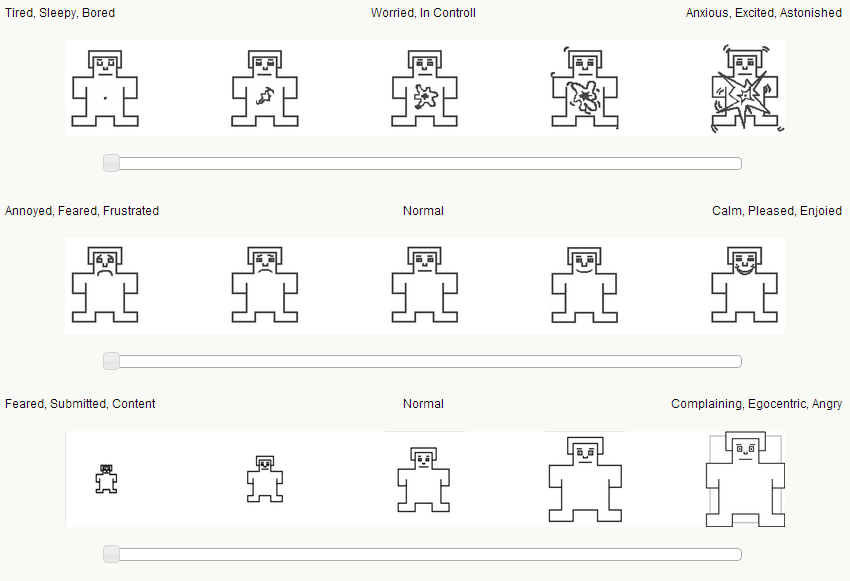
\includegraphics[width=0.7\textwidth]{images/sam.png}
  \label{fig:sam}
\end{figure}

\paragraph{Intrinsic Motivation Inventory}

Different components of game experience were measured using the Intrinsic Motivation Inventory questionnaire \cite{?}. It combines several game-related subjective measurement dimensions: interest/enjoyment, perceived competence, effort and felt pressure and tension while playing the game. Each one of these components consists of ?? question items (e.g., ``While playing, I was thinking about how much I enjoyed it'' is a interest/enjoyment component item). Question items were shown in a randomized order every time the page was viewed. Each question item consists of a statement on a five-point scale ranging from 1 (strongly disagreeing with the statement) to 5 (strongly agreeing with the statement). The questionnaire was developed based on survey studies \cite{?}.

\paragraph{Player Experience of Need Satisfaction}


\paragraph{Game Engagement Questionnaire}

%%%%%%%%%%%%%nasty%%%%%%%%%%%%%
An image of a regular participant signal values is depicted at
the following. In this image from left to right the light blue line
shows different conditions being played, and when the light blue
line is declining towards its base value, that is the period that
participant is asked to stop playing and instead relaxing and filling
out the questionnaires. The blue line is the normalized GSR signal
value of the participants which is used as an estimation of his
excitement level. The yellow green and pink lines are showing the
three different modes of Player, NPC and Environment parameters
being adapted

Following image is the GSR signal of players playing different
conditions from 1 to 4. From left to right the conditions are the
Default, Player, NPC and the Environment mode. This signals are all
based to an initial start value of 100, during the play experience,
some of them had gone bellow the start point and some other had risen
above that. Also the start time for each different condition is
shifted 500 seconds times the number of condition, from 0.

The following image is the average of GSR values for players in four
different conditions from left to right: Default, Player, NPC and
Environment modes
%%%%%%%%%%%%%nasty%%%%%%%%%%%%%

\section{Results}


% describe 16 participant's feedbacks and comments, and general ideas on how each one of them migh have experienced different situations through the game.


%------------------------------------------------------------------------------

\chapter{Discussion}
\label{chap:discus}

%5 to 10 pages
%talk for the discussion
%State what you've done and what you've found
%Summarize contributions (achievements and impact)
%Outline open issues/directions for future work

%------------------------------------------------------------------------------

% Bibliography
\uofsbibliography[plain]{content/bibliography}

%------------------------------------------------------------------------------

% APPENDICES
\uofsappendix
\chapter{Transforming physiological variables into arousal-valence space} \label{app:phys-to-av}    
The following 22 rules were used as described in Section ~\ref{subsec:fuzzi} to transform physiological variables into arousal-valence space:

\begin{lstlisting}[language=python]
if (GSR      is high     )                        then (arousal is high     )
if (GSR      is mid-high )                        then (arousal is mid-high )
if (GSR      is mid-low  )                        then (arousal is mid-low  )
if (GSR      is low      )                        then (arousal is low      )
if (HR       is low      )                        then (arousal is low      )
if (HR       is high     )                        then (arousal is high     )
if (EMGfrown is high     )                        then (valence is very low )
if (EMGfrown is mid      )                        then (valence is low      )
if (EMGsmile is mid      )                        then (valence is high     )
if (EMGsmile is high     )                        then (valence is very high)
if (GSR      is low      ) and (HR is high)       then (arousal is midlow   )
if (GSR      is high     ) and (HR is low )       then (arousal is midhigh  )
if (GSR      is high     ) and (HR is mid )       then (arousal is high     )
if (GSR      is mid-high ) and (HR is mid )       then (arousal is mid-high )
if (GSR      is mid-low  ) and (HR is mid )       then (arousal is mid-low  )
if (EMGsmile is low      ) and (EMGfrown is low ) then (valence is neutral  )
if (EMGsmile is high     ) and (EMGfrown is low ) then (valence is very high)
if (EMGsmile is high     ) and (EMGfrown is mid ) then (valence is high     )
if (EMGsmile is low      ) and (EMGfrown is high) then (valence is very low )
if (EMGsmile is mid      ) and (EMGfrown is high) then (valence is low      )
if (EMGsmile is low      ) and (EMGfrown is low ) and (HR is low)  then (valence is low)
if (EMGsmile is low      ) and (EMGfrown is low ) and (HR is high) then (valence is high)
\end{lstlisting}

\chapter{Transforming arousal-valence space into emotional states}        \label{app:av-to-emotion} 
The following 67 rules were used as described in Section ~\ref{subsec:fuzzi} to convert arousal and valence into boredom, challenge, excitement, frustration, and fun:

\begin{enumerate}
\item If (arousal is not veryLow) and (valence is midHigh) then (fun is low)
\item If (arousal is not low) and (valence is midHigh) then (fun is low)
\item If (arousal is not veryLow) and (valence is high) then (fun is medium)
\item If (valence is veryHigh) then (fun is high)
\item If (arousal is midHigh) and (valence is midLow) then (challenge is low)
\item If (arousal is midHigh) and (valence is midHigh) then (challenge is low)
\item If (arousal is high) and (valence is midLow) then (challenge is medium)
\item If (arousal is high) and (valence is midHigh) then (challenge is medium)
\item If (arousal is veryHigh) and (valence is midLow) then (challenge is high)
\item If (arousal is veryHigh) and (valence is midHigh) then (challenge is high)
\item If (arousal is midLow) and (valence is midLow) then (boredom is low)
\item If (arousal is midLow) and (valence is low) then (boredom is medium)
\item If (arousal is low) and (valence is low) then (boredom is medium)
\item If (arousal is low) and (valence is midLow) then (boredom is medium)
\item If (arousal is midLow) and (valence is veryLow) then (boredom is high)
\item If (arousal is low) and (valence is veryLow) then (boredom is high)
\item If (arousal is veryLow) and (valence is veryLow) then (boredom is high)
\item If (arousal is veryLow) and (valence is low) then (boredom is high)
\item If (arousal is veryLow) and (valence is midLow) then (boredom is high)
\item If (arousal is midHigh) and (valence is midLow) then (frustration is low)
\item If (arousal is midHigh) and (valence is low) then (frustration is medium)
\item If (arousal is high) and (valence is low) then (frustration is medium)
\item If (arousal is high) and (valence is midLow) then (frustration is medium)
\item If (arousal is midHigh) and (valence is veryLow) then (frustration is high)
\item If (arousal is high) and (valence is veryLow) then (frustration is high)
\item If (arousal is veryHigh) and (valence is veryLow) then (frustration is high)
\item If (arousal is veryHigh) and (valence is low) then (frustration is high)
\item If (arousal is veryHigh) and (valence is midLow) then (frustration is high)
\item If (valence is veryLow) then (fun is veryLow)(challenge is veryLow)
\item If (valence is low) then (fun is veryLow)(challenge is veryLow)
\item If (valence is high) then (challenge is veryLow)(boredom is veryLow)(frustration is veryLow)
\item If (valence is veryHigh) then (challenge is veryLow) (boredom is veryLow)(frustration is veryLow)
\item If (valence is midHigh) then (boredom is veryLow) (frustration is veryLow)
\item If (arousal is veryLow) then (challenge is veryLow) (frustration is veryLow)
\item If (arousal is low) then (challenge is veryLow)(frustration is veryLow)
\item If (arousal is midLow) then (challenge is veryLow) (frustration is veryLow)
\item If (arousal is midHigh) then (boredom is veryLow)
\item If (arousal is high) then (boredom is veryLow)
\item If (arousal is veryHigh) then (boredom is veryLow)
\item If (arousal is veryLow) and (valence is midHigh) then (fun is veryLow)
\item If (arousal is low) and (valence is midHigh) then (fun is veryLow)
\item If (arousal is veryLow) and (valence is high) then (fun is low)
\item If (valence is midLow) then (fun is veryLow)
\item If (arousal is veryLow) and (valence is high) then (boredom is low)
\item If (arousal is low) and (valence is midHigh) then (boredom is low)
\item If (arousal is veryLow) and (valence is midHigh) then (boredom is medium)
\item If (arousal is veryHigh) and (valence is veryLow) then (challenge is medium)
\item If (arousal is veryHigh) and (valence is veryHigh) then (challenge is medium)
\item If (arousal is high) and (valence is low) then (challenge is low)
\item If (arousal is high) and (valence is high) then (challenge is low)
\item If (arousal is veryHigh) and (valence is low) then (challenge is high)
\item If (arousal is veryHigh) and (valence is high) then (challenge is high)
\item If (arousal is midHigh) and (valence is midHigh) then (excitement is low)
\item If (arousal is high) and (valence is midHigh) then (excitement is medium)
\item If (arousal is high) and (valence is high) then (excitement is medium)
\item If (arousal is midHigh) and (valence is high) then (excitement is medium)
\item If (arousal is veryHigh) and (valence is midHigh) then (excitement is high)
\item If (arousal is veryHigh) and (valence is high) then (excitement is high)
\item If (arousal is veryHigh) and (valence is veryHigh) then (excitement is high)
\item If (arousal is high) and (valence is veryHigh) then (excitement is high)
\item If (arousal is midHigh) and (valence is veryHigh) then (excitement is high)
\item If (arousal is midLow) then (excitement is veryLow)
\item If (arousal is low) then (excitement is veryLow)
\item If (arousal is veryLow) then (excitement is veryLow)
\item If (valence is veryLow) then (excitement is veryLow)
\item If (valence is low) then (excitement is veryLow)
\item If (valence is midLow) then (excitement is veryLow)
\end{enumerate}

\chapter{Demographics Questionnaire}                                      \label{app:q-dmg}         \box{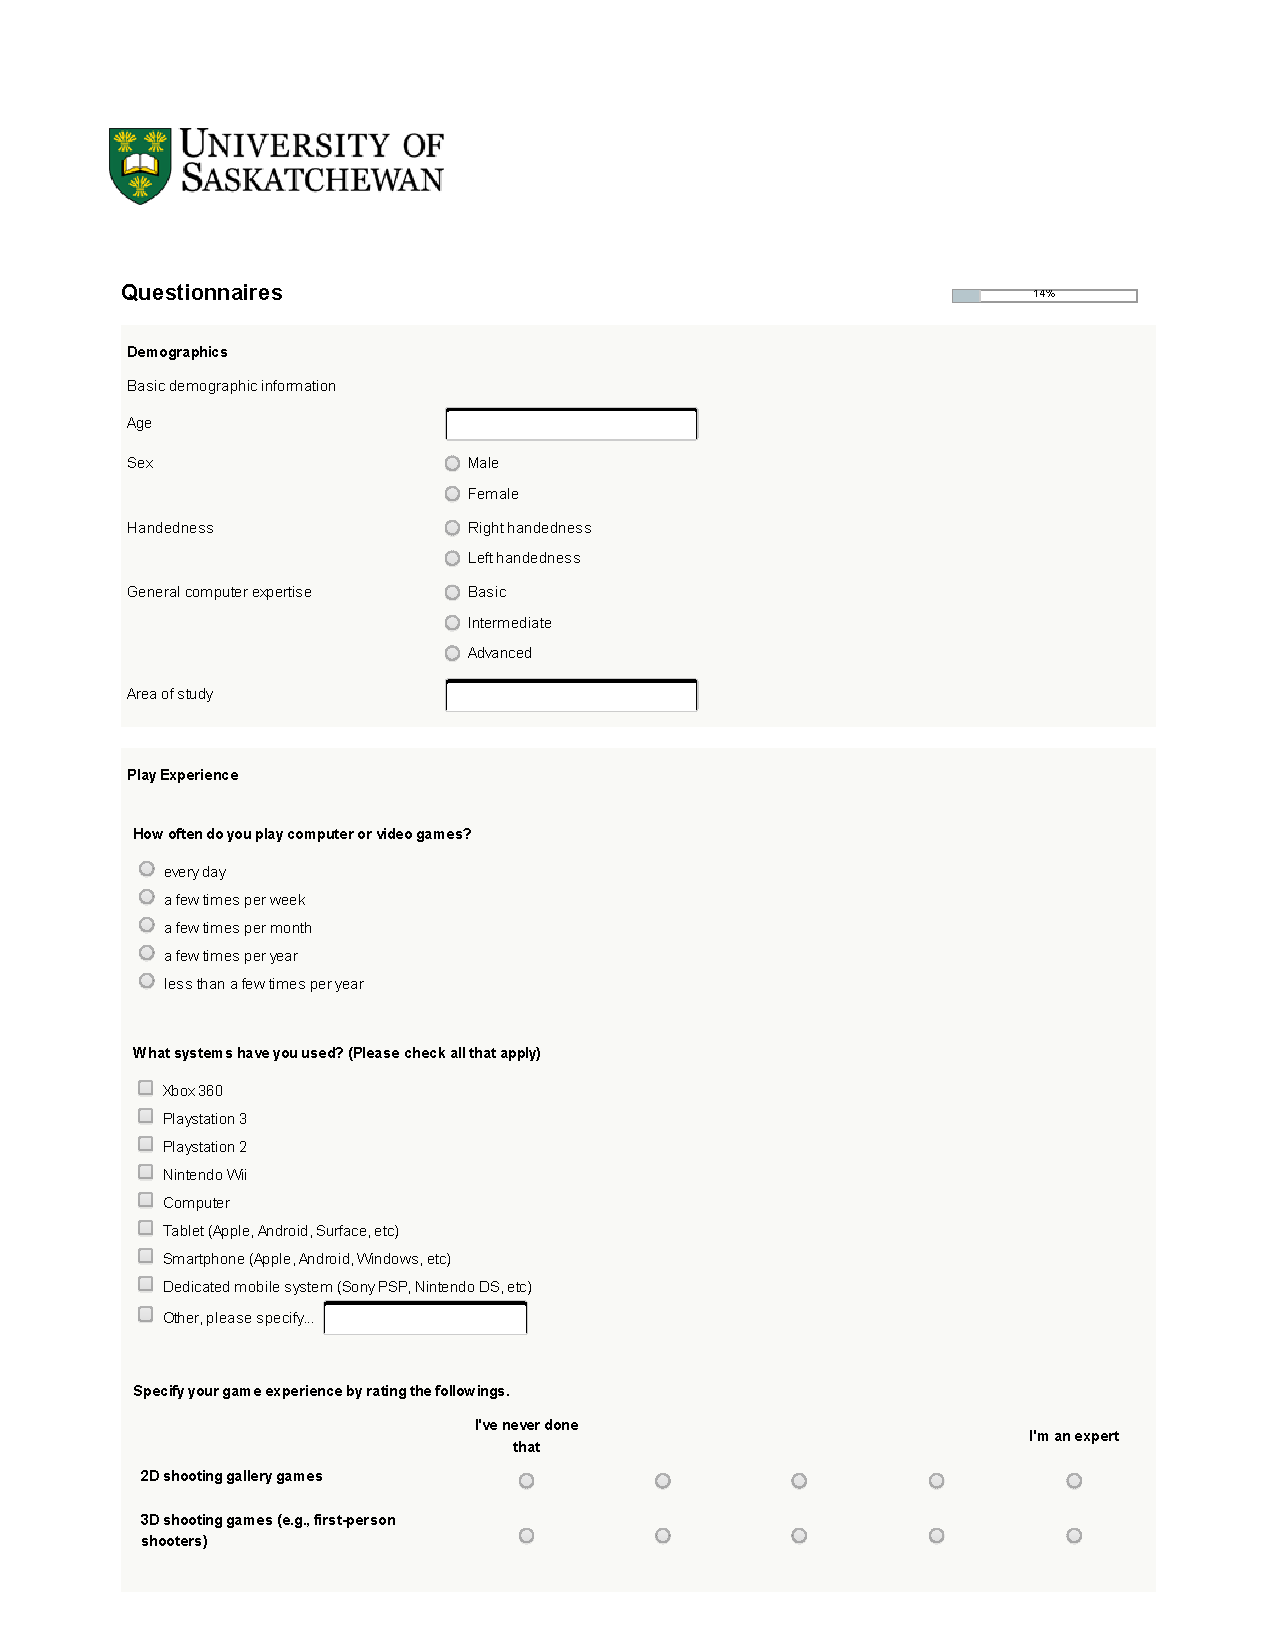
\includegraphics[page=1]{content/q-dmg.pdf}}
                                                                                                    \includepdf[pages={2}]{content/q-dmg.pdf}
                                                                                                    \box{\includegraphics[page=3]{content/q-dmg.pdf}}
\chapter{Condition Questionnaire}                                         \label{app:q-cnd}         \box{
\includegraphics[page=1]{content/q-cnd.pdf}}
\chapter{Self-Assessment-Manikin Arousal Scales Questionnaire}            \label{app:q-sam}         \box{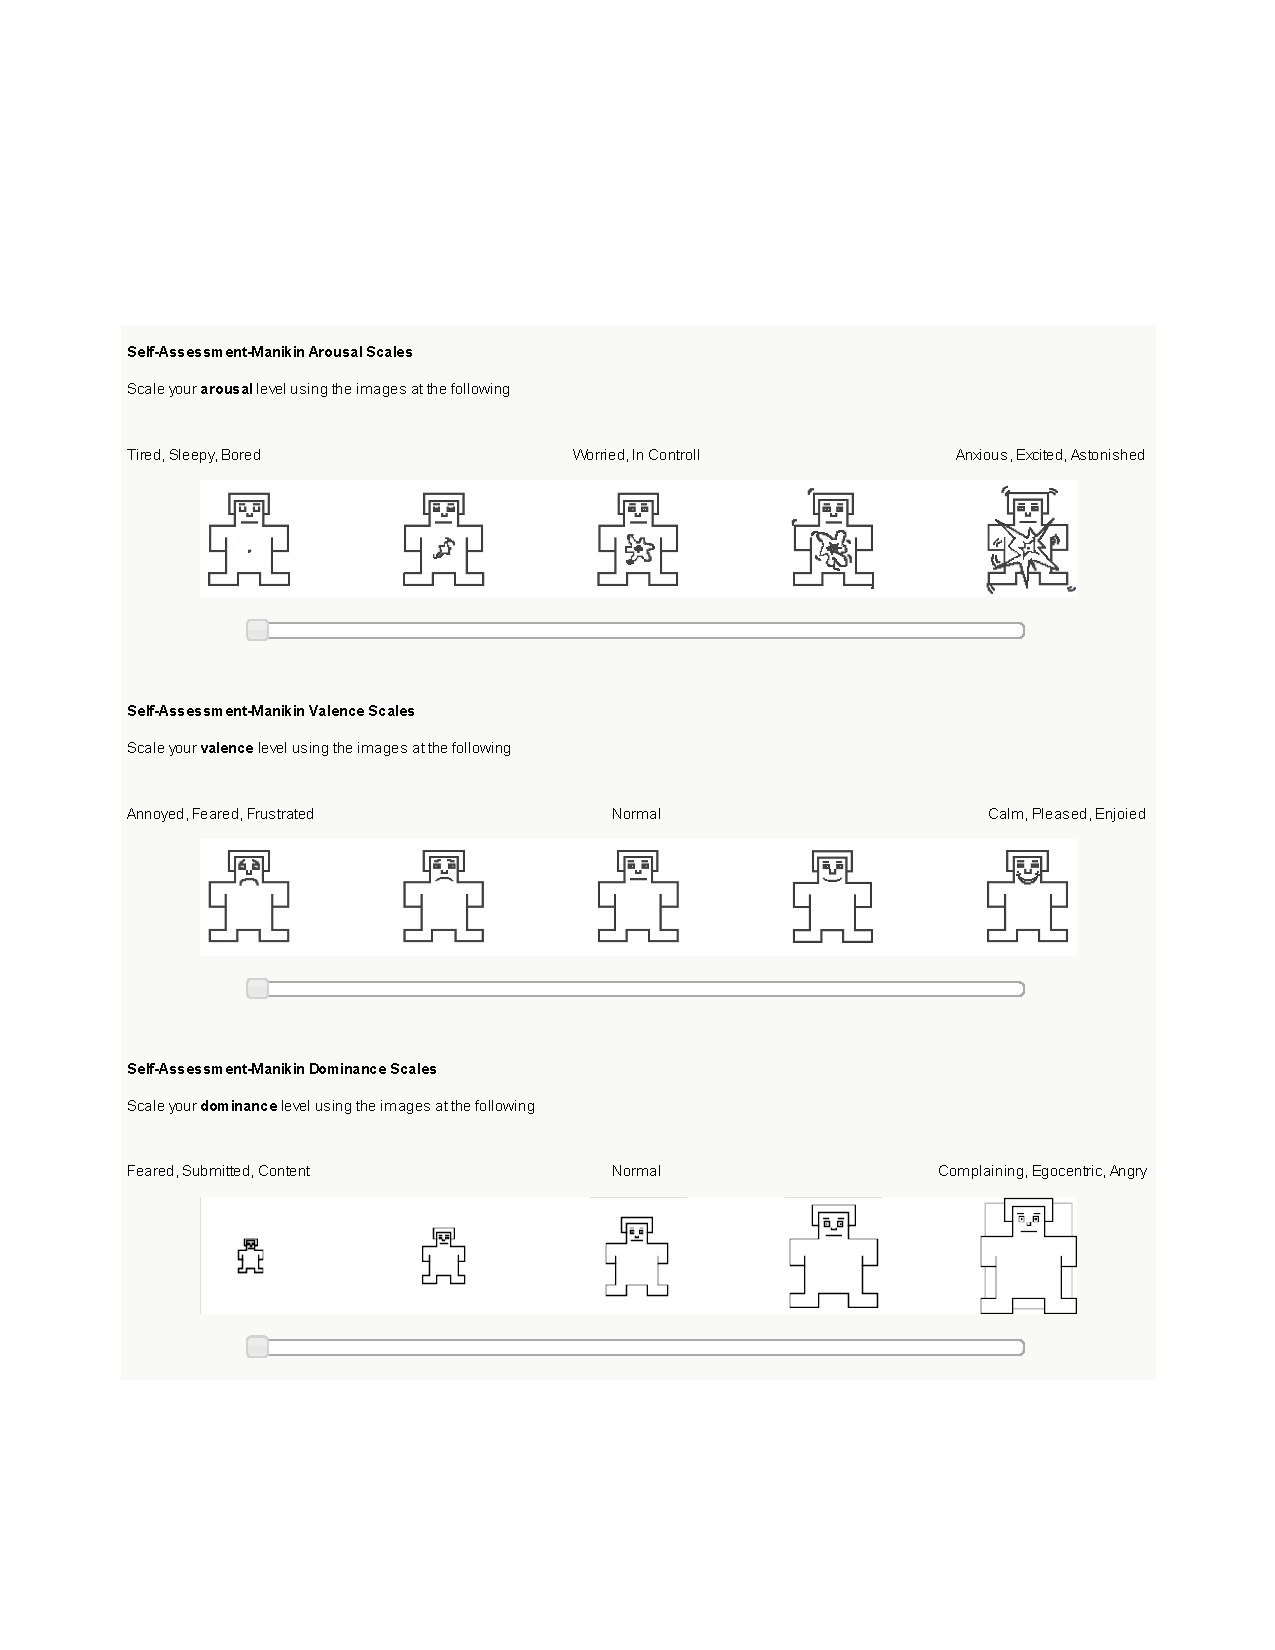
\includegraphics[page=1]{content/q-sam.pdf}}
\chapter{Intrinsic Motivation Inventory Questionnaire}                    \label{app:q-ini}         \box{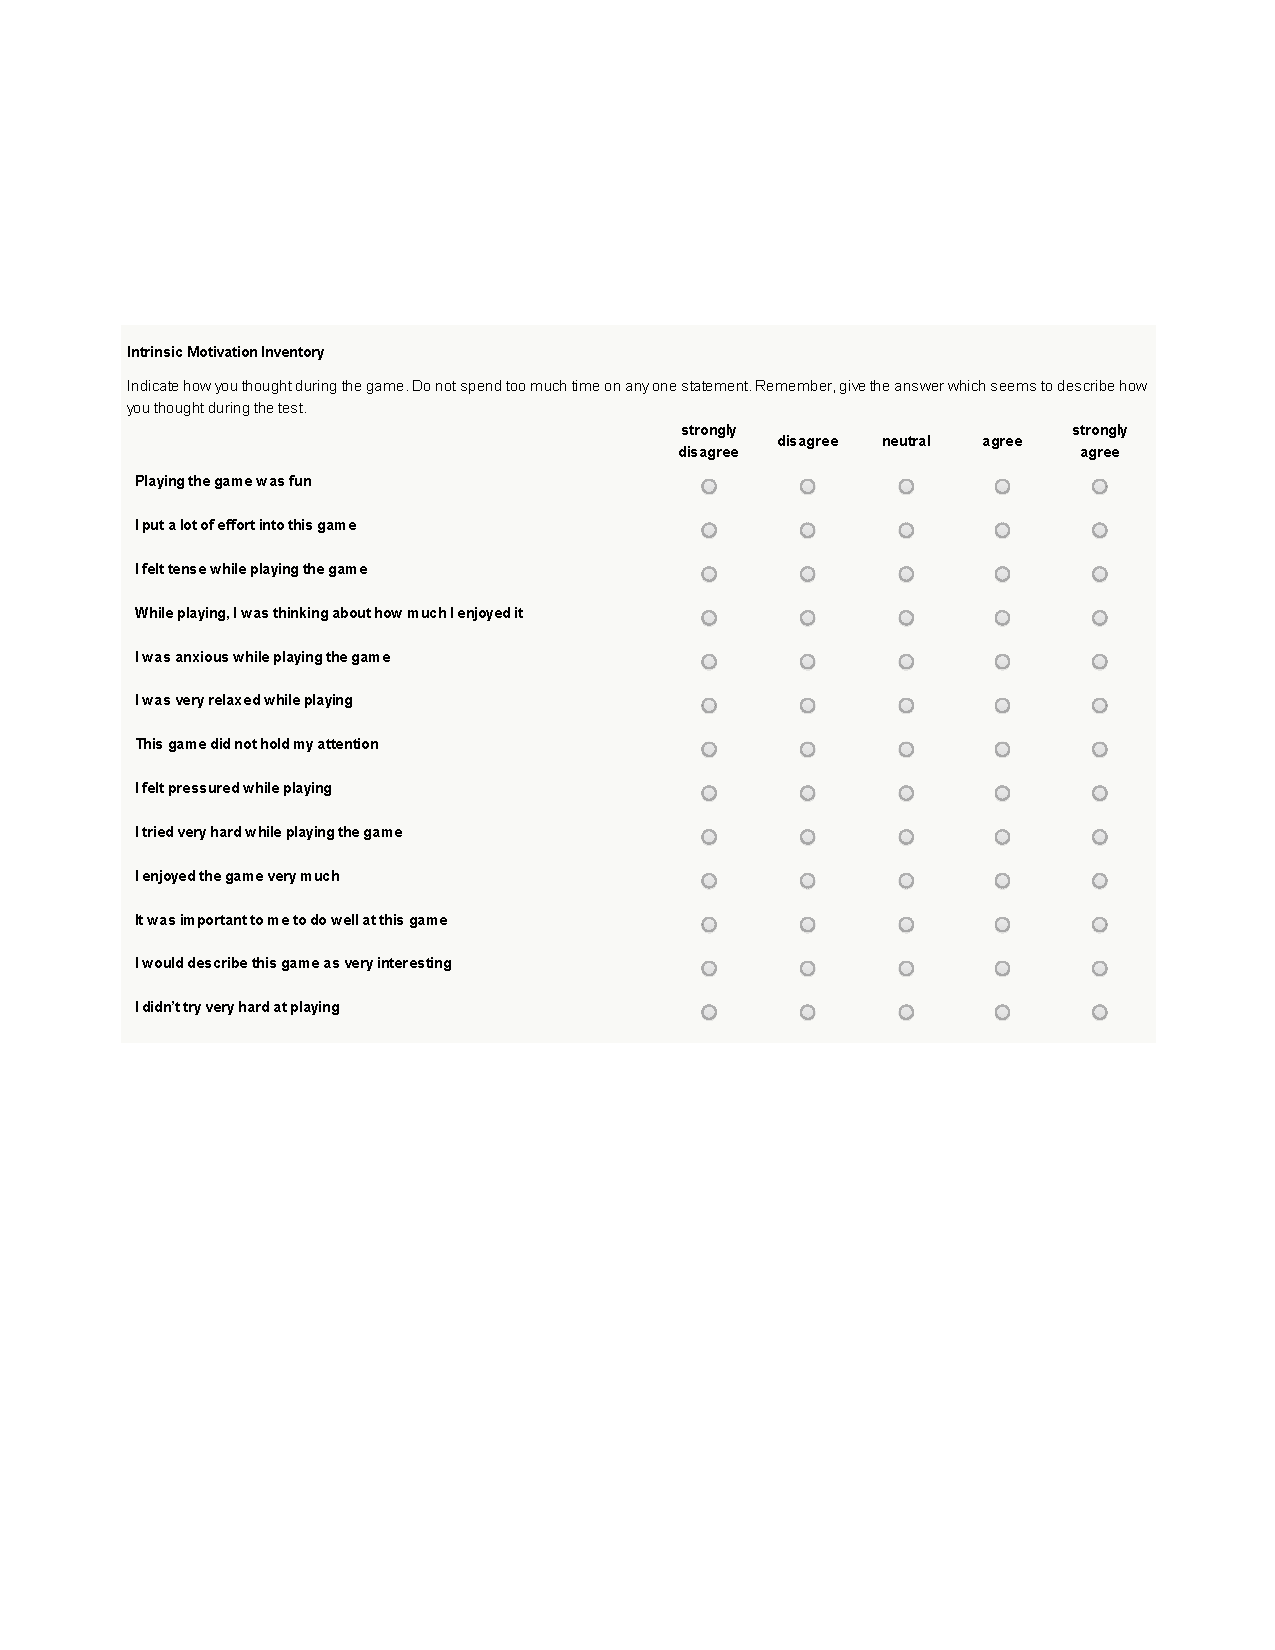
\includegraphics[page=1]{content/q-imi.pdf}}
\chapter{Player Experience of Need Satisfaction Questionnaire}            \label{app:q-pens}        \box{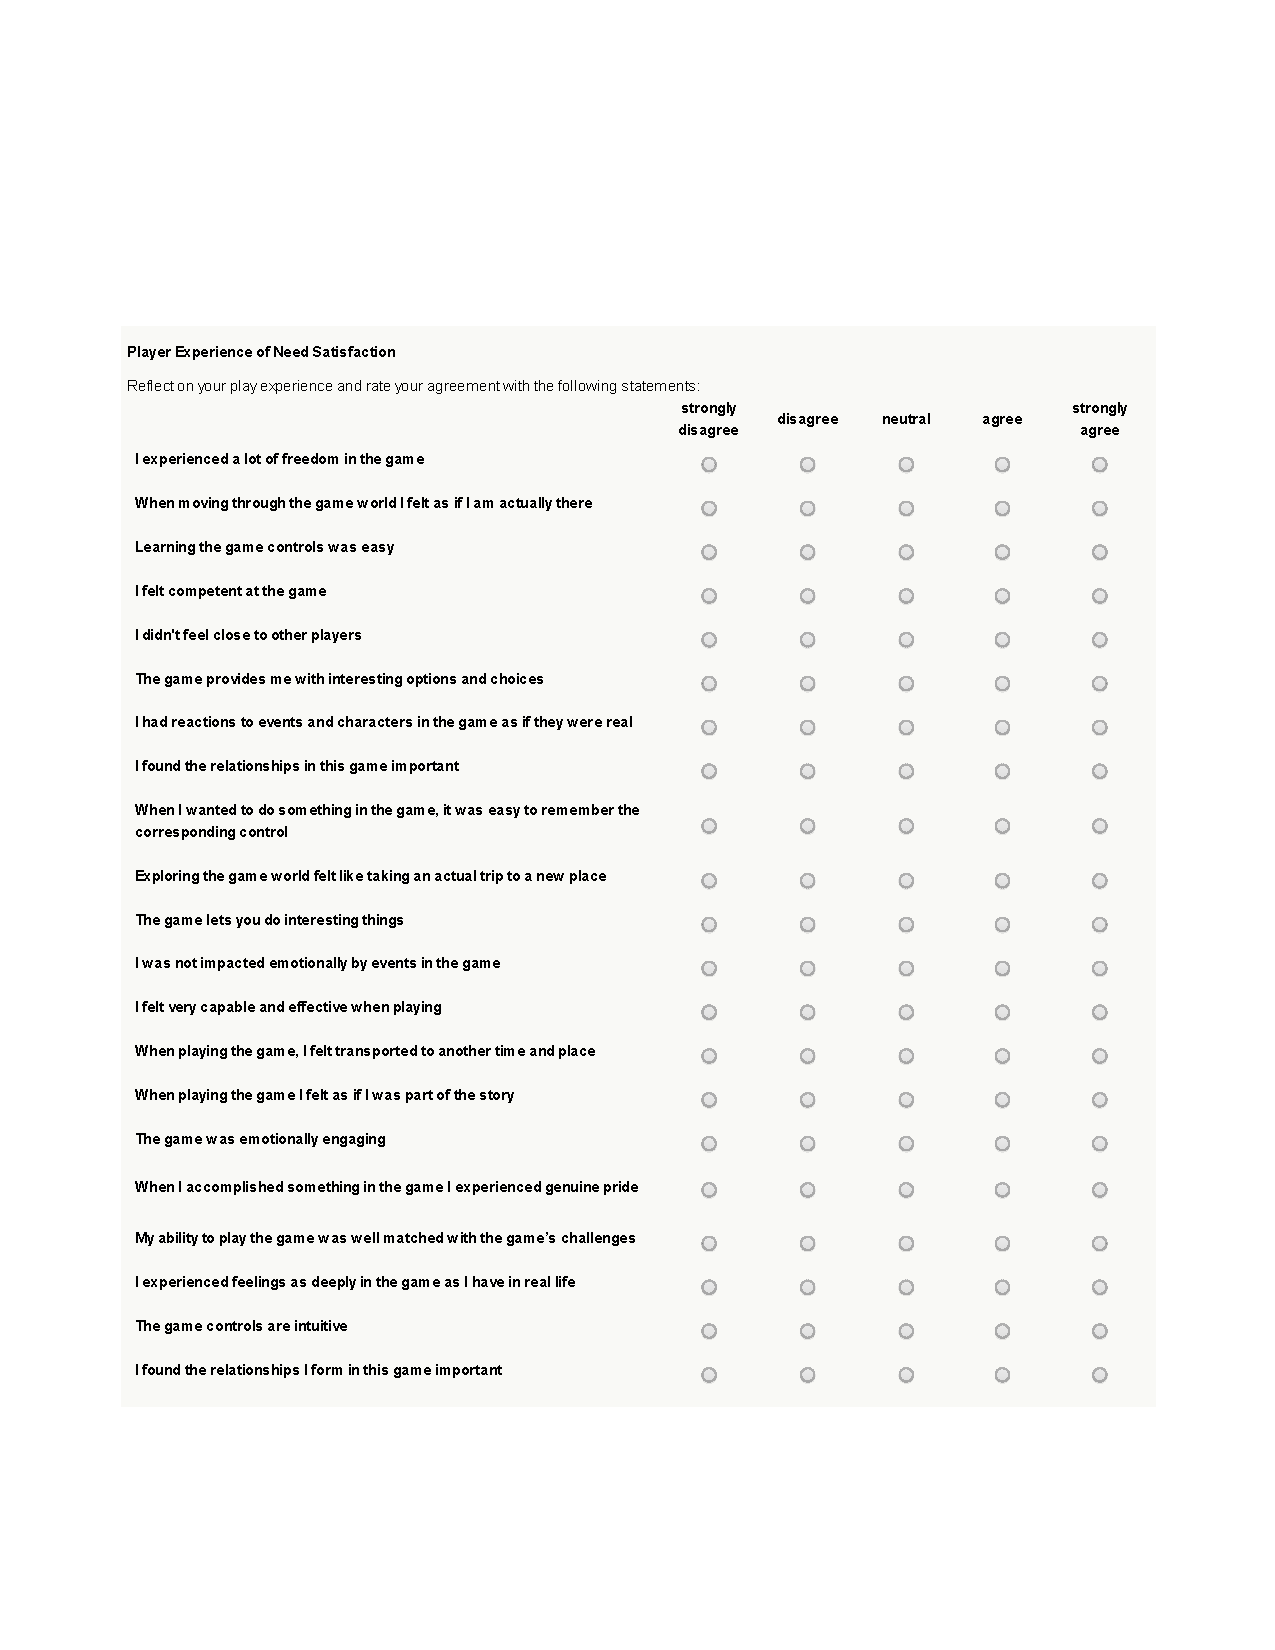
\includegraphics[page=1]{content/q-pens.pdf}}
\chapter{Game Engagement Questionnaire}                                   \label{app:q-geq}         \box{
\includegraphics[page=1]{content/q-geq.pdf}}

%------------------------------------------------------------------------------

\end{document}

%------------------------------------------------------------------------------
